\documentclass[11pt,a4paper]{article}
\usepackage[utf8]{inputenc}
\usepackage[ngerman]{babel}
\usepackage{csquotes}
\usepackage{hyperref}
\usepackage{tabularx}
\usepackage{calc}
\usepackage{geometry}
\usepackage[scaled]{helvet}
\usepackage[T1]{fontenc}
\usepackage{float}
\usepackage{graphicx}


\renewcommand{\familydefault}{\sfdefault}

\geometry{
  left=1.5cm,
  right=1.5cm,
  top=1.5cm,
  bottom=1.5cm,
  includeheadfoot
}

% Schriftgrößen und Titeldefinitionen
\newcommand{\titleformat}{\fontsize{18pt}{22pt}\selectfont}
\newcommand{\sectionformat}{\fontsize{14pt}{18pt}\selectfont}
\newcommand{\subsectionformat}{\fontsize{11pt}{14pt}\selectfont}
\newcommand{\bodytextformat}{\fontsize{10pt}{12pt}\selectfont}


\begin{document}

\begin{flushleft}
    {\titleformat\textbf{Integration einer Sprachsteuerungsfunktion in Mobile Apps}}\\[0.5cm]
  \end{flushleft}

\bodytextformat

\noindent
\begin{tabularx}{\linewidth}{@{}p{4cm}X@{}}
    \textbf{Themenbereiche:} & Sprachsteuerung, Audio, Machine Learning, Triggerwort-Erkennung, Mobile Apps \\
    \textbf{Studierender:} & Ruben Nuñez \\
    \textbf{Dozent:} & Dr. Florian Herzog \\
    \textbf{Experte:} & Damien Piguet \\
    \textbf{Auftraggeber:} & Stefan Reinhard \\
    \textbf{Keywords:} & Sprachsteuerung, Mobile Apps, Machine Learning, Triggerwort-Erkennung, Audioverarbeitung, Datensatzerstellung, Modelltraining, App-Integration \\
\end{tabularx}
    




\section{Aufgabenstellung}
Die Bachelorarbeit zielt darauf ab, eine Sprachsteuerungsfunktion für mobile Apps zu entwickeln, wobei der Fokus auf der Erkennung von Triggerwörtern in akustischer Sprache liegt. Zentrale Aspekte sind die Entwicklung eines Machine Learning-Modells, seine Implementierung in eine mobile Plattform wie iOS und die Beachtung von Datenschutz und ethischen Richtlinien beim Erstellen und Verwenden eines Datensatzes.


\section{Ergebnisse}
Im Rahmen Bachelorarbeit wurden folgende Ergebnisse erzielt:

\begin{itemize}
    \itemsep0em
    \item Ein \textbf{Machine Learning-Modell}, das in der Lage ist, Triggerwörter in akustischer Sprache zu erkennen.
    \item Eine \textbf{Integration in eine iOS-App}, die das Modell verwendet, um Triggerwörter in Echtzeit zu erkennen.
    \item Ein \textbf{Datensatz}, welcher ethische Richtlinien und Datenschutzbestimmungen einhält welcher für das Training des Modells verwendet wurde.
    \item Eine \textbf{Dokumentation}, die die Entwicklung des Modells, die Erstellung des Datensatzes und die Implementierung der App beschreibt.
\end{itemize}

\noindent
Beim Machine Learning Modell handelt es sich um eine Kombination aus einem Convolutional Neural Network (CNN) und einem LSTM-Netzwerk (Long Short-Term Memory). Das CNN wird verwendet, um die akustischen Merkmale der Sprache zu extrahieren, während das LSTM-Netzwerk die zeitlichen Abhängigkeiten zwischen den akustischen Merkmalen erfasst. Das Modell wurde in PyTorch implementiert und mit dem erstellten Datensatz. Das Modell wurde mit dem erstellten Datensatz trainiert und erreichte eine Accuracy von 0.88 und eine F1-Score von 0.80 auf dem Testdatensatz. Das Modell hat den Name \textbf{WakeupTriggerConvLSTM2s} und ist in der Lage, Triggerwörter in Echtzeit zu erkennen. Eine Transformationskomponente mit dem Namen \textbf{AudioToSpectrogramTransformJit} zur Umwandlung von Audio in Spektrogramme wurde ebenfalls in PyTorch entwickelt und dient als Feature-Extraktions-Modul. \\

\noindent
Ein kritischer Aspekt für die Lösungsakzeptanz war die Gewährleistung der Effizienz des Modells bezogen auf die Real-Time-Fähigkeit. Das Modell erzielt eine Vorhersagegeschwindigkeit von 0.01 Sekunden pro Spektrogramm und erfüllt damit die Anforderungen an eine Echtzeiterkennung, ohne die Geräteleistung zu beeinträchtigen. Die nachfolgende Abbildung zeigt schematisch den Aufbau der Verarbeitungskette in der App.\\

\begin{figure}[H]
	\centering
	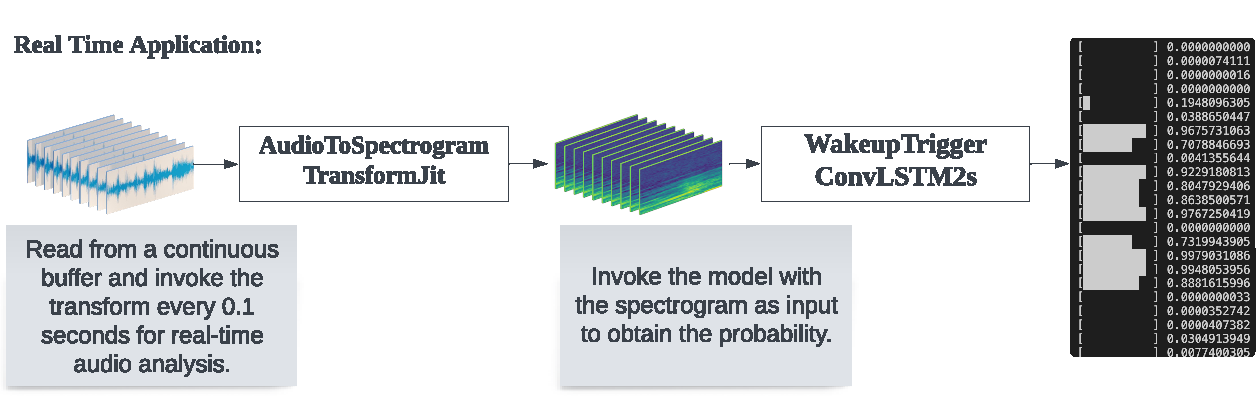
\includegraphics[width=0.8\linewidth, trim=0pt 10pt 0pt 15pt, clip]{img/realtime-application.pdf}
	\caption{Real Time Anwendung}
\end{figure}

\noindent
Die realisierte Applikation wurde als iOS App implementiert und verwendet die entwickelten PyTorch Module \textit{AudioToSpectrogramTransformJit} und \textit{WakeupTriggerConvLSTM2s}.





\section{Lösungskonzept}


\section{Spezielle Herausforderungen}


\section{Ausblick}


\end{document}
